\documentclass[tikz,border=4pt]{standalone}
\usepackage{libertine}
\usetikzlibrary{arrows.meta,calc,positioning,fit,backgrounds,shapes.geometric}
\definecolor{paperink}{HTML}{263441}
\definecolor{papermuted}{HTML}{647481}
\definecolor{paperline}{HTML}{CCD5DB}
\definecolor{paperblue}{HTML}{2D5F91}
\definecolor{paperbluefill}{HTML}{EFF5FA}
\definecolor{paperorange}{HTML}{B66731}
\definecolor{paperorangefill}{HTML}{FCF4EB}
\definecolor{papergreen}{HTML}{3F7558}
\definecolor{papergreenfill}{HTML}{EFF6F1}
\tikzset{
  papertext/.style={font=\footnotesize, text=paperink},
  papermini/.style={font=\scriptsize, text=papermuted},
  paneltitle/.style={font=\footnotesize\bfseries, text=paperink},
  bluebox/.style={draw=paperblue, fill=paperbluefill, rounded corners=1pt,
    line width=.6pt, font=\footnotesize, text=paperink, align=center,
    inner xsep=6pt, inner ysep=5pt},
  orangebox/.style={draw=paperorange, fill=paperorangefill, rounded corners=1pt,
    line width=.6pt, font=\footnotesize, text=paperink, align=center,
    inner xsep=6pt, inner ysep=5pt},
  greenbox/.style={draw=papergreen, fill=papergreenfill, rounded corners=1pt,
    line width=.6pt, font=\footnotesize, text=paperink, align=center,
    inner xsep=6pt, inner ysep=5pt},
  graybox/.style={draw=paperline, fill=white, rounded corners=1pt,
    line width=.6pt, font=\footnotesize, text=paperink, align=center,
    inner xsep=6pt, inner ysep=5pt},
  orangeflow/.style={-{Stealth[length=2mm]}, draw=paperorange, line width=1pt},
  blueflow/.style={-{Stealth[length=2mm]}, draw=paperblue, line width=1.15pt},
  greenflow/.style={-{Stealth[length=2mm]}, draw=papergreen, line width=1pt},
  grayflow/.style={-{Stealth[length=1.8mm]}, draw=papermuted, line width=.65pt}
}

\begin{document}
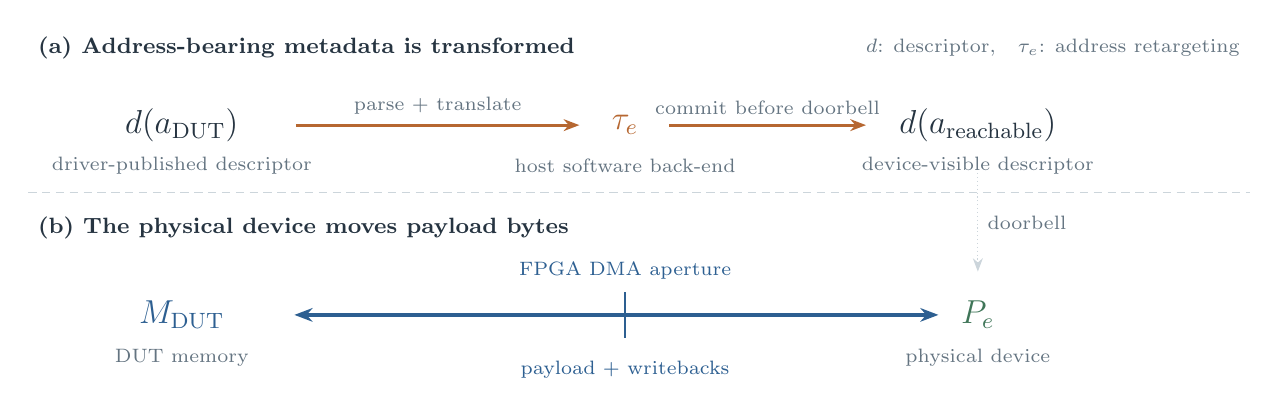
\begin{tikzpicture}[x=1cm,y=1cm]
  % Metadata transformation and byte movement are separate operations.
  \node[paneltitle, anchor=west] at (.22,4.53) {(a) Address-bearing metadata is transformed};
  \draw[paperline, densely dashed] (.22,2.69) -- (15.74,2.69);
  \node[font=\large, text=paperink] at (2.17,3.55) {$d(a_{\mathrm{DUT}})$};
  \node[papermini] at (2.17,3.03) {driver-published descriptor};
  \node[font=\large, text=paperorange] at (7.80,3.55) {$\tau_e$};
  \node[papermini] at (7.80,3.03) {host software back-end};
  \node[font=\large, text=paperink] at (12.28,3.55) {$d(a_{\mathrm{reachable}})$};
  \node[papermini] at (12.28,3.03) {device-visible descriptor};
  \draw[orangeflow] (3.62,3.55) -- node[papermini, above] {parse + translate} (7.22,3.55);
  \draw[orangeflow] (8.36,3.55) -- node[papermini, above] {commit before doorbell} (10.86,3.55);
  \node[papermini, anchor=east] at (15.73,4.53) {$d$: descriptor,\quad $\tau_e$: address retargeting};

  \node[paneltitle, anchor=west] at (.22,2.24) {(b) The physical device moves payload bytes};
  \node[font=\large, text=paperblue] at (2.17,1.14) {$M_{\mathrm{DUT}}$};
  \node[papermini] at (2.17,.60) {DUT memory};
  \node[font=\large, text=papergreen] at (12.28,1.14) {$P_e$};
  \node[papermini] at (12.28,.60) {physical device};
  \draw[paperblue, line width=1.5pt,
    {Stealth[length=2.3mm]}-{Stealth[length=2.3mm]}]
    (3.60,1.14) -- (11.78,1.14);
  \draw[paperblue, line width=1pt] (7.80,.85) -- (7.80,1.43);
  \node[papermini, above, text=paperblue] at (7.80,1.47) {FPGA DMA aperture};
  \node[papermini, text=paperblue] at (7.80,.44) {payload + writebacks};
  \draw[paperline, densely dotted, -{Stealth[length=1.7mm]}]
    (12.28,2.94) -- node[papermini, right] {doorbell} (12.28,1.69);
\end{tikzpicture}
\end{document}
